\documentclass[12pt, a5paper, french]{memoir}
\usepackage[bottom=91pt]{geometry}
\usepackage[utf8]{inputenc}
\usepackage[T1]{fontenc}
\usepackage{lmodern}
\usepackage{microtype}
\usepackage{dramatist}
\usepackage[modulo]{lineno}
\usepackage{hyperref}
\usepackage{graphicx}
\usepackage{babel}

\renewcommand{\actname}{Acte}
\renewcommand{\scenename}{Scène}
\renewcommand{\printscenenum}{\scenenumfont \thescene}
\renewcommand{\casttitlename}{Personnages}

\makepagestyle{myps}
\makeevenfoot{myps}{\thepage}{}{}
\makeoddfoot{myps}{}{}{\thepage}

\title{L'anneau de Gygès}
\author{Alexandre \textsc{Pachot}\thanks{Texte sous licence \href{http://creativecommons.org/licenses/by-sa/4.0/deed.fr}{CC BY-SA}, inspiré d’une fable racontée dans la \textit{République} de Platon.}}

\hyphenation{Michel-angelo}

\begin{document}
\maketitle
\vfill
\begin{figure}[h]
\centering
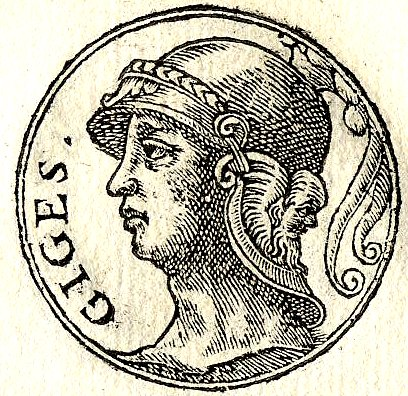
\includegraphics[scale=1]{Gyges.jpg}
\end{figure}
\vfill
\thispagestyle{empty}
\newpage
\renewcommand\contentsname{Sommaire}
\tableofcontents*

\Character[Gygès]{Gygès}{G}
\Character[Candaule, le roi]{Candaule}{R}
\Character[Nyssia, la fiancée du roi]{Nyssia}{r}
\Character[Laurel, un serviteur du roi]{Laurel}{S}
\Character[Hardy, un serviteur de Nyssia]{Hardy}{s}
\Character[Bonnie, une voleuse]{Bonnie}{Vi}
\Character[Clyde, un voleur]{Clyde}{Vj}
\Character[Leonardo, un berger]{Leonardo}{Bi}
\Character[Donatello, un berger]{Donatello}{Bj}
\Character[Michelangelo, un berger]{Michelangelo}{Bk}
\Character[Raffaello, un berger]{Raffaello}{Bl}
\Character[Tiziano, un berger]{Tiziano}{Bm}
   
\DramPer*
\pagestyle{myps}
\linenumbers
\scene

\StageDir{\G, \Vi, \Vj}
\begin{drama}
\Vispeaks Connais-tu la dernière nouvelle ?
\Vjspeaks Quelle nouvelle ?
\Vispeaks Le roi vient de s’acheter la dernière Nintendo, la 3DS~XXL.
\Vjspeaks Comment sais-tu ça ?
\Vispeaks C’est écrit dans le journal. Si seulement tu savais lire\dots
\Vjspeaks Pff ! Le journal, il suffit de le regarder à la télé !
\Vispeaks Au lieu de dire des bêtises, dis-moi plutôt comment on va faire pour voler cette console.
\Vjspeaks \direct{Apercevant quelqu’un au loin.} C’est qui là-bas ?
\Vispeaks C’est Gygès, au pied de son arbre, en train de surveiller ses chèvres.
\Vjspeaks Allons le saluer. \direct{À Gygès.} Gygès, tu viens avec nous, on va élaborer un plan pour dérober la dernière console du roi.
\Gspeaks Moi, Monsieur, je suis honnête, je respecte les lois, je ne vole pas.
\Vispeaks Gygès, au lieu de faire le malin, réponds plutôt à la question suivante : tu ne voles pas, car tu as peur de te faire arrêter, ou parce que tu es l’incarnation même de la justice ? Si tu avais de super-pouvoirs tout en étant certain de ne pas te faire attraper, que ferais-tu ? Respecterais-tu la loi, ou pas ? Là, tu fais moins le malin ! Bon, je te laisse, moi j’ai du travail à faire, il faut qu’on trouve un plan pour s’emparer de cette console !

\scene

\StageDir{\G}
\Gspeaks \direct{Scrutant le pied de l’arbre.} Un affaissement ? Je ne l’avais jamais remarqué. On dirait qu’il y a quelque chose au fond. Tiens, une boite ? Il y a un texte écrit dessus : \og Ô mortel, garde-toi d’envier le bonheur d’aucun autre homme. \fg{} \direct{Ouvre la boite.} Tout cela pour un anneau ! \direct{Passe la bague à son doigt, le chaton à l’extérieur.} Bon, rien ne se passe ! Ce n’est pas tout, mais il faut que je retourne au village, il y a le conseil des bergers.

\scene

\StageDir{\G, \Bi, \Bj, \Bk, \Bl, \Bm}
\Bispeaks \direct{Apercevant Gygès} Gygès, dépêche-toi, cela fait des lustres qu’on t’attend. On n’a pas que ça à faire. J’ai des pommes de terre à éplucher.
\Bjspeaks Oh ! On est ici pour parler de chèvres, pas de patates !
\Bkspeaks Bon. Qui va voir le roi pour faire un rapport sur l'état des troupeaux ?
\Blspeaks Pas moi.
\Bmspeaks Moi.
\Bjspeaks Non, pas toi. La dernière fois, tu as eu un problème avec le roi.
\Bispeaks Bon, alors c’est Gygès qui va aller voir le roi.
\Gspeaks \direct{À lui-même.} Je vais tourner le chaton de ma bague vers l’intérieur, voir ce que cela fait.
\Bispeaks Il est où Gygès ? Saperlipopette, il a encore disparu.
\Blspeaks C’est vrai, ça. Il était encore là, il y a 5~secondes.
\Gspeaks \direct{Tournant le chaton vers l’extérieur.} Les amis, c’est moi que vous cherchez ?
\Bmspeaks Ah ! Te voilà enfin de retour. Bon, nous avons décidé que c’est toi qui vas aller voir le roi pour lui faire un rapport sur nos troupeaux.
\Gspeaks D’accord, je m’en vais de ce pas, voir le roi.

\scene

\StageDir{\G, \R, \r, \S}
\Sspeaks Votre Majesté, Gygès vient d’arriver.
\Rspeaks Bien, faites-le entrer.
\Gspeaks Votre Majesté.
\Rspeaks Gygès, mon ami, comment vont les affaires ?
\Gspeaks Bien.
\Rspeaks Avant de parler affaires, il faut que je te présente ma nouvelle fiancée. Passe un peu de temps avec elle et dis-moi ce que tu en penses.
\Gspeaks Votre Majesté, cela serait indécent\dots
\Rspeaks J’insiste. \direct{À Nyssia.} Nyssia, viens voir ici. Je dois partir, j’ai des affaires à régler. Je te présente Gygès, un ami qui va te tenir compagnie pour le diner.

\scene

\StageDir{\G, \r, \s}
\Gspeaks \direct{À lui-même.} J’ai bien mangé. Il en a de la chance le roi, d’épouser une si belle fille. Je l’envie.
\sspeaks \direct{À Nyssia.} Mon altesse, je viens d’apprendre que le roi est furieux de la conduite de Gygès. Il veut le tuer.
\rspeaks Vite, va prévenir Gygès du sort qui l’attend.
\sspeaks \direct{À Gygès.} Monsieur, vous courez un grand danger, le roi veut votre mort.
\Gspeaks Ha ! Le scélérat ! Je vais utiliser mon anneau d’invisibilité pour le tuer pendant son sommeil.

\scene

\StageDir{\Vi, \Vj}
\Vispeaks Connais-tu la dernière nouvelle ?
\Vjspeaks Quelqu’un a volé la console du roi ?
\Vispeaks Non ! Le roi a été assassiné. Maintenant, c’est Gygès qui est roi à la place du roi.
\Vjspeaks Le roi est mort, vive le roi !
\Vispeaks Mais cela ne répond pas à la question.
\Vjspeaks Quelle question ?
\Vispeaks Si l’on était protégé de la conséquence de nos actes, est-ce qu’on agirait de la même manière ?
\end{drama}

\hfill
\centering

\textsc{Fin}
\end{document}